\documentclass[11pt,a4paper]{article}
\usepackage[T1]{fontenc}
\usepackage[margin=2.3cm]{geometry}
\usepackage{amsmath,amssymb}
\usepackage{graphicx}
\usepackage[dvipsnames]{xcolor}
\usepackage{enumitem}
\usepackage[colorlinks=true,linkcolor=blue,urlcolor=blue]{hyperref}
\setlength{\parskip}{0.6em}
\setlength{\parindent}{0pt}
\begin{document}

\begin{center}{\LARGE\bfseries opencomfort}\\[0.4em]{\large Cool a building passively with shading and ventilation, in three sessions.}\\[0.2em]\small PAN IIT OSS explainer \textbullet{} higher secondary to diploma / undergraduate (levels 4-5)\end{center}

\section*{Why this exists}
Shading and ventilation can keep a building cool without much energy. This explainer follows the idea from the heat balance of a hot room to the sun's position, the shadow of a sunshade, the air flow through open windows and an hour-by-hour simulation of a room with a sunlit roof and thermal mass, using only school geometry, the energy balance and a few textbook formulas.

\section*{The end goal}
Cool a building passively with shading and ventilation. The end goal is to know where the heat in a hot room comes from, size a sunshade and the window openings for a real room, and show with a validated simulation which combination of shade, roof colour, ventilation and thermal mass keeps it comfortable, at what cost. The same ideas apply to schools, hostels, offices and factory sheds.

\section*{How the three sessions build up}
\begin{enumerate}[nosep]
\item \textbf{Session 1: Where the heat in a hot room comes from} (Level 1, conceptual interactive model, 60 min).
\item \textbf{Session 2: Size a sunshade and a breeze} (Level 2, mathematical engineering model, 75 min).
\item \textbf{Session 3: Simulate a hot day and choose a passive design} (Level 3, simulation and validation, 90 min).
\end{enumerate}

\textit{This is a simplified educational model. It is not a validated design tool and must not be used for real structures, electrical installations, vehicles, industrial processes or medical decisions.}

\section{Session 1: Where the heat in a hot room comes from}

\subsection*{A. Real-world problem}
On an April afternoon in Chennai a closed top-floor room with a sunny west window can feel hotter than the street outside. Where does that heat come from? And why do two old, cheap ideas, a sunshade (chajja) over the window and open windows, make such a big difference without using any electricity? (General education only: this is a simplified model, not a building design method.)

\subsection*{B. Concept and theory}
Heat always flows from hot to cold. A room gains heat in four ways. \textbf{Conduction} through a wall, roof or glass of area A gives Q = U A dT, where the U-value says how many watts pass through 1 m2 for each kelvin of difference (230 mm brick about 2, bare concrete roof about 2.5, single glass about 5 W/(m2 K)). \textbf{Sunshine} through a window brings Q = SHGC A I, where I is the sunshine on the glass in W/m2 and the solar heat gain coefficient SHGC (about 0.8 for clear glass) is the share that becomes heat; a shade outside that blocks a fraction s of the sun multiplies this by (1 - s). \textbf{People and equipment} add their heat directly (about 75 W per resting adult). \textbf{Air flow} replaces indoor air with outdoor air: with ACH air changes per hour in a room of volume Vol, the flow is V\_dot = ACH Vol / 3600 and the heat it brings is rho cp V\_dot (T\_out - T\_in), with rho cp = 1200 J/(m3 K). If nothing changes for a long time the room settles where all the flows add to zero. Then the indoor temperature is the outdoor temperature plus the gains divided by everything that lets heat out. Shading shrinks the top of that fraction; ventilation grows the bottom.

\begin{itemize}[nosep]
\item U: U-value (thermal transmittance) of a wall, roof or window (W/(m2 K))
\item A: area of a surface or window (m2)
\item UA: sum of U x A over all outside surfaces (W/K)
\item I: sunshine falling on the window (irradiance) (W/m2)
\item SHGC: solar heat gain coefficient of the glass (no unit)
\item s: fraction of the sun blocked by a shade (no unit)
\item ACH: air changes per hour (1/h)
\item H\_v: ventilation conductance rho cp V\_dot (W/K)
\item T\_out, T\_in: outdoor and indoor air temperature (C)
\end{itemize}

\begin{equation*}
Q_{\mathrm{cond}} = U A\,(T_{\mathrm{out}} - T_{\mathrm{in}})
\end{equation*}

\begin{equation*}
Q_{\mathrm{sun}} = (1 - s)\,\mathrm{SHGC}\,A_{\mathrm{win}}\,I
\end{equation*}

\begin{equation*}
H_v = \rho c_p \dot V = 1200 \times \frac{\mathrm{ACH} \times \mathrm{Vol}}{3600}
\end{equation*}

\begin{equation*}
T_{\mathrm{in}} = T_{\mathrm{out}} + \frac{Q_{\mathrm{sun}} + Q_{\mathrm{int}}}{UA + H_v}
\end{equation*}

\begin{center}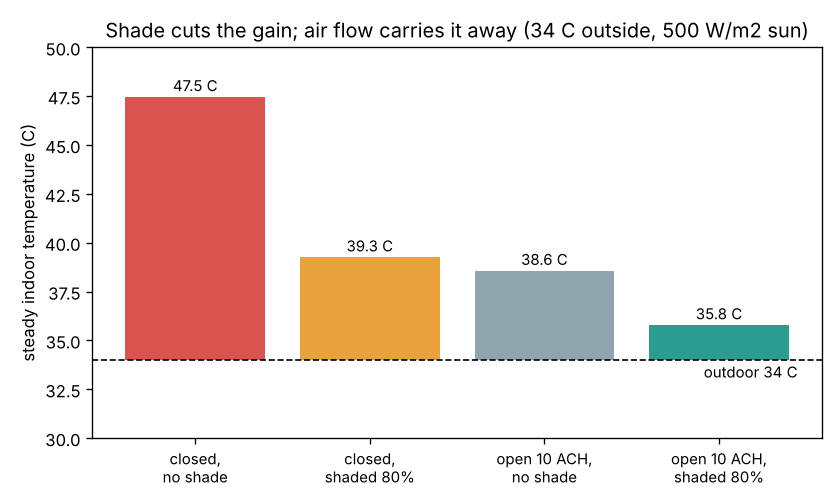
\includegraphics[width=0.85\linewidth]{figures/s01_steady_designs.png}\\\small Steady indoor temperature for four designs: shading and ventilation together bring the room to 35.8 C.\end{center}

\subsection*{E. Worked example}
The example room (UA = 70 W/K, 48 m3, 250 W of internal gains) has 500 W/m2 of sun on its 2 m2 window (SHGC 0.8) at 34 C outside. A shade blocks 80 percent of the sun and the windows give 10 air changes per hour. Find the steady indoor temperature and check the energy balance.
\begin{enumerate}[nosep]
\item Sun gain: Q\_sun = (1 - 0.8) x 0.8 x 2 x 500 = 160 W.
\item Air flow: V\_dot = 10 x 48 / 3600 = 0.1333 m3/s, so H\_v = 1200 x 0.1333 = 160 W/K.
\item Steady temperature: T\_in = 34 + (160 + 250) / (70 + 160) = 34 + 410 / 230 = 35.78 C.
\item Check: walls and roof carry 70 x 1.78 = 125 W out, air carries 160 x 1.78 = 285 W out; 125 + 285 = 410 W = gains.
\item Without shade or air flow (0.5 ACH from leaks, H\_v = 8 W/K): T\_in = 34 + 1050 / 78 = 47.5 C.
\end{enumerate}
\textbf{Answer.} About 35.8 C, 1.8 K above outdoor; the closed, unshaded room would sit at 47.5 C.

\subsection*{F. Questions}
\begin{enumerate}[nosep]
\item \textbf{Conceptual.} Why does a shade work much better outside the window than a curtain inside it?
\item \textbf{Numerical.} A 1.5 m2 clear window (SHGC 0.8) receives 600 W/m2. How much heat enters with no shade and with a shade blocking 70 percent? Check the units.
\item \textbf{Graph and simulation interpretation.} In the second figure, why do both curves flatten as the air change rate grows, and what temperature do they approach?
\item \textbf{Design and optimisation challenge.} Design: the example room must stay within 2 K of outdoor at 34 C with 500 W/m2 on the window. Find the minimum air changes per hour with no shade and with an 80 percent shade. Which is more realistic to achieve?
\end{enumerate}

\section{Session 2: Size a sunshade and a breeze}

\subsection*{A. Real-world problem}
In Session 1 we simply assumed that a shade blocks 80 percent of the sun and that open windows give 10 air changes per hour. A builder needs real numbers: how deep must the concrete sunshade (chajja) over a west window in Chennai be, and how much air will two open windows move on a breezy evening? (Simplified clear-sky and textbook ventilation formulas; not a design method.)

\subsection*{B. Concept and theory}
The sun's position comes from three angles. The \textbf{declination} delta is the latitude where the sun is overhead today; it swings between +23.45 degrees in June and -23.45 degrees in December. The \textbf{hour angle} omega is 15 degrees per hour away from solar noon. The \textbf{altitude} alpha above the horizon follows from sin(alpha) = sin(phi) sin(delta) + cos(phi) cos(delta) cos(omega), with phi the latitude; the \textbf{azimuth} (compass direction) follows from the same angles. In Chennai (13.08 N) the sun is north of overhead at noon from late April to mid-August, so south windows get almost no direct sun in summer. For a vertical wall facing azimuth psi, the \textbf{wall-solar azimuth} gamma is the sun's azimuth minus psi, and the beam strikes the glass with cos(theta) = cos(alpha) cos(gamma). Seen in a section through the wall, the sun's rays slope at the \textbf{profile angle} Omega with tan(Omega) = tan(alpha) / cos(gamma). An overhang of depth D, a gap G above a window of height H, shades the fraction f = (D tan(Omega) - G) / H of the window (clipped to 0..1). A high sun has a steep profile angle and is easy to block; the low afternoon sun on a west wall is very hard to block. For air flow, wind presses on the windward wall and sucks on the leeward one; the difference of pressure coefficients dCp is about 0.8. Two openings in series act like one effective opening A\_eff, and the flow is Q = Cd A\_eff U sqrt(dCp) with discharge coefficient Cd about 0.6. With only one window the flow is roughly Q = 0.025 A U. Warm indoor air is lighter, so a low and a high opening a height h apart drive a \textbf{stack} flow Q = Cd A\_eff sqrt(2 g h dT / T\_mean).

\begin{itemize}[nosep]
\item phi: latitude (Chennai 13.08 N) (degrees)
\item delta, omega: declination, hour angle (degrees)
\item alpha, az: sun altitude, sun azimuth from north (degrees)
\item gamma: wall-solar azimuth (sun azimuth minus wall azimuth) (degrees)
\item Omega: profile (vertical shadow) angle (degrees)
\item D, G, H: overhang depth, gap above window, window height (m)
\item U, dCp, Cd: wind speed, pressure coefficient difference, discharge coefficient (m/s, no unit, no unit)
\item Q, A\_eff: air flow, effective opening area (m3/s, m2)
\end{itemize}

\begin{equation*}
\delta = 23.45^\circ \sin\!\left(360^\circ\,\frac{284 + n}{365}\right),\qquad \omega = 15^\circ\,(t - 12)
\end{equation*}

\begin{equation*}
\sin\alpha = \sin\phi\,\sin\delta + \cos\phi\,\cos\delta\,\cos\omega
\end{equation*}

\begin{equation*}
\tan\Omega = \frac{\tan\alpha}{\cos\gamma},\qquad f = \mathrm{clip}\!\left(\frac{D\tan\Omega - G}{H},\,0,\,1\right)
\end{equation*}

\begin{equation*}
Q_{\mathrm{wind}} = C_d\,A_{\mathrm{eff}}\,U\,\sqrt{\Delta C_p},\qquad \frac{1}{A_{\mathrm{eff}}^2} = \frac{1}{A_1^2} + \frac{1}{A_2^2}
\end{equation*}

\begin{equation*}
Q_{\mathrm{stack}} = C_d\,A_{\mathrm{eff}}\,\sqrt{\frac{2 g h\,\Delta T}{T_{\mathrm{mean}}}},\qquad \mathrm{ACH} = \frac{3600\,Q}{\mathrm{Vol}}
\end{equation*}

\begin{center}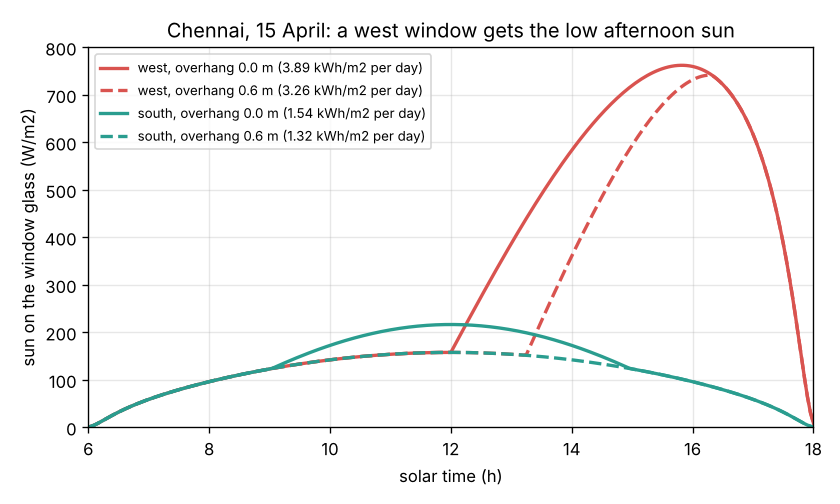
\includegraphics[width=0.85\linewidth]{figures/s02_window_sun.png}\\\small Sun on a west and a south window over the day, with and without a 0.6 m overhang.\end{center}

\subsection*{E. Worked example}
Chennai (13.08 N), 15 April (day 105), 3 pm solar time. Find the sun's altitude, the overhang depth that fully shades a 1.5 m high west window with a 0.3 m gap, and the shaded fraction for a 0.6 m overhang. Then find the air changes in a 48 m3 room with two 0.5 m2 openings and a 1.5 m/s wind.
\begin{enumerate}[nosep]
\item Declination: delta = 23.45 sin(360 x 389 / 365) = 9.41 degrees. Hour angle omega = 15 x 3 = 45 degrees.
\item sin(alpha) = 0.2263 x 0.1636 + 0.9741 x 0.9865 x 0.7071 = 0.7165, so alpha = 45.8 degrees; the azimuth is 270.1 (due west), so gamma is about 0 and the profile angle is also 45.8 degrees.
\item Full shade: D = (G + H) / tan(Omega) = 1.8 / 1.028 = 1.75 m.
\item A 0.6 m overhang: f = (0.6 x 1.028 - 0.3) / 1.5 = 0.21, only 21 percent of the window.
\item A\_eff = 0.5 / sqrt(2) = 0.354 m2; Q = 0.6 x 0.354 x 1.5 x sqrt(0.8) = 0.285 m3/s; ACH = 3600 x 0.285 / 48 = 21.3.
\end{enumerate}
\textbf{Answer.} Altitude 45.8 degrees; a 1.75 m overhang shades the whole window but a 0.6 m one only 21 percent; cross ventilation gives about 21 air changes per hour.

\subsection*{F. Questions}
\begin{enumerate}[nosep]
\item \textbf{Conceptual.} Why is a horizontal overhang good for a south window in Chennai in winter, but nearly useless for a west window at 4 pm?
\item \textbf{Numerical.} On the equinox (declination 0) at solar noon, what is the sun's altitude in Chennai (13.08 N)? Which way does it face?
\item \textbf{Graph and simulation interpretation.} In the first figure, why does the west window's sunshine stay low until noon and then rise sharply, while the 0.6 m overhang only delays the rise?
\item \textbf{Design and optimisation challenge.} Design: a 48 m3 bedroom needs at least 15 air changes per hour from cross ventilation with a 1.0 m/s evening breeze. Two equal openings on opposite walls are allowed. What is the smallest area for each opening? What if only one wall can have an opening?
\end{enumerate}

\section{Session 3: Simulate a hot day and choose a passive design}

\subsection*{A. Real-world problem}
Session 1 gave one steady temperature for fixed conditions, and Session 2 the sun and the air flow at one moment. But the sun moves, the outdoor air swings from 26.5 C at dawn to 35.5 C in the afternoon, the roof bakes in the sun, and the floor slab soaks up heat by day and gives it back at night. Can we step through a whole day, check the simulation against Session 1 and the energy balance, and then choose the cheapest set of passive measures (sunshade, white roof, night ventilation) that keeps a top-floor room in Chennai comfortable on 15 April? (A simplified teaching model, not a design tool.)

\subsection*{B. Concept and theory}
A sunlit roof is far hotter than the air. Its effect on the room is as if the air above it were at the \textbf{sol-air temperature} T\_sa = T\_out + a I\_roof / h\_o - 3.9 K, where a is the roof's solar absorptance (about 0.8 for dark concrete, 0.3 for a white lime or reflective coating), I\_roof the sunshine on the roof and h\_o = 20 W/(m2 K); the 3.9 K is heat the roof radiates to the cold sky. The room has two parts. The \textbf{air} stores very little heat, so at every moment its heat flows balance: walls and glass (UA\_w), roof (UA\_r, driven by T\_sa), ventilation (H\_v), the \textbf{thermal mass} (hA, the floor slab and inner walls at T\_m) and the gains add to zero, which makes the air temperature a weighted average. The \textbf{mass} has a large heat capacity C\_m and changes slowly: C\_m dT\_m/dt = hA (T\_a - T\_m) + f Q\_sun, where f = 0.7 is the share of the window sun that lands on the floor. We step this equation every 5 minutes with Runge-Kutta 4. We want the day that repeats itself (a periodic steady state); because the model is linear, two trial days give it exactly. \textbf{Night flushing} opens the windows from 7 pm to 7 am, when outdoor air is cooler, to cool the mass; then the windows are shut by day so the cool mass absorbs the afternoon heat. People in naturally ventilated buildings adapt to their climate: the \textbf{adaptive comfort} model (ASHRAE Standard 55) puts the 80 percent acceptability upper limit at 0.31 T\_pma + 17.8 + 3.5 C, which is 30.9 C for a prevailing mean outdoor temperature of 31 C, and a ceiling fan moving air at about 0.9 m/s raises it by 1.8 K to 32.7 C. \textbf{Discomfort degree-hours} add up the kelvin above that limit over the hours of the day.

\begin{itemize}[nosep]
\item T\_a, T\_m: indoor air temperature, thermal-mass temperature (C)
\item T\_sa: sol-air temperature of the roof (C)
\item a: solar absorptance of the roof surface (no unit)
\item UA\_w, UA\_r: conductance of walls plus glass, of the roof (W/K)
\item C\_m, hA: heat capacity of the mass, air-to-mass conductance (J/K, W/K)
\item H\_v: ventilation conductance 1200 x ACH x Vol / 3600 (W/K)
\item T\_lim: adaptive comfort upper limit (C)
\item DH: discomfort degree-hours above T\_lim (K h)
\end{itemize}

\begin{equation*}
T_{\mathrm{sa}} = T_{\mathrm{out}} + \frac{a\,I_{\mathrm{roof}}}{h_o} - 3.9
\end{equation*}

\begin{equation*}
T_a = \frac{(UA_w + H_v)\,T_{\mathrm{out}} + UA_r\,T_{\mathrm{sa}} + hA\,T_m + Q_{\mathrm{int}} + (1-f)\,Q_{\mathrm{sun}}}{UA_w + UA_r + H_v + hA}
\end{equation*}

\begin{equation*}
C_m\,\frac{dT_m}{dt} = hA\,(T_a - T_m) + f\,Q_{\mathrm{sun}}
\end{equation*}

\begin{equation*}
T_{\mathrm{lim}} = 0.31\,T_{\mathrm{pma}} + 17.8 + 3.5\ (+1.8\ \text{with a fan})
\end{equation*}

\begin{equation*}
\mathrm{DH} = \int \max(0,\ T_a - T_{\mathrm{lim}})\,dt
\end{equation*}

\begin{center}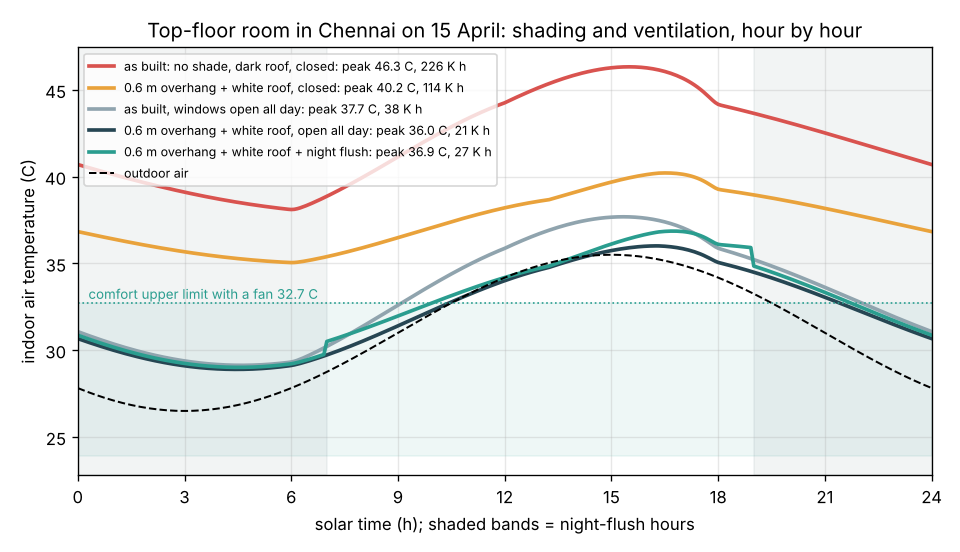
\includegraphics[width=0.85\linewidth]{figures/s03_day_designs.png}\\\small Indoor air temperature over 15 April for five designs, with the comfort limit.\end{center}

\subsection*{E. Worked example}
For the as-built room at 15:00 on 15 April, find the outdoor temperature and the sol-air temperature of the dark roof. Then validate the simulation: with constant inputs (34 C outside and on the roof, 160 W of sun, 10 air changes per hour) it must give the Session 1 answer.
\begin{enumerate}[nosep]
\item Outdoor: T\_out = 31 + 4.5 cos(0) = 35.5 C.
\item Sun on the roof at 15:00: altitude 45.8 degrees, beam 1100 exp(-0.18 / 0.7165) = 856 W/m2, so I\_roof = 856 x (0.7165 + 0.12) = 716 W/m2.
\item Sol-air: T\_sa = 35.5 + 0.8 x 716 / 20 - 3.9 = 60.2 C for the dark roof, and 35.5 + 0.3 x 716 / 20 - 3.9 = 42.3 C for a white roof.
\item Validation: with constant inputs the mass stops changing, so T\_a = 34 + (160 + 250) / (70 + 160) = 35.78 C at every step, which the simulation reproduces to 10\textasciicircum{}-6 K. Its mass sits 0.7 x 160 / 400 = 0.28 K warmer, because it absorbs the floor sun.
\item Energy check on the real day: heat flowing in over 24 h minus heat stored in the mass is at most 0.02 percent of the heat flows, and the mass ends the day at its starting temperature.
\end{enumerate}
\textbf{Answer.} T\_out = 35.5 C, roof sol-air 60.2 C (dark) or 42.3 C (white); the simulation reproduces Session 1 exactly and conserves energy.

\subsection*{F. Questions}
\begin{enumerate}[nosep]
\item \textbf{Conceptual.} In the design-day results, opening the windows all day beats night flushing (36.0 C against 36.9 C). When would night flushing win, and why?
\item \textbf{Numerical.} Find the sol-air temperature of a flat roof at noon when the outdoor air is 34.2 C and the sun on the roof is 1027 W/m2, for a dark roof (a = 0.8) and a white roof (a = 0.3). How much hotter than the air is each?
\item \textbf{Graph and simulation interpretation.} In Figure 1, why does the as-built room reach its peak around 15:30 and stay above 38 C all night, while the outdoor air falls to 26.5 C?
\item \textbf{Design and optimisation challenge.} Design: using \texttt{choose\_design}, find the cheapest package that keeps discomfort under 25 K h, and the cheapest under 20 K h. Explain why the roof coating comes before the overhang for this room.
\end{enumerate}

\section{Real-world mini-project}
\textbf{Choose the passive cooling package for a top-floor room.} A family wants their top-floor bedroom in Chennai (the Session 3 room) to stay comfortable with a ceiling fan on hot April days, without buying an air conditioner. The options, with illustrative costs: a concrete overhang over the west window of 0.6 m (Rs 6000) or 1.2 m (Rs 12000), a white reflective roof coating that lowers the absorptance from 0.8 to 0.3 (Rs 8000), and keeping windows open all day (free) or opening them only at night with insect mesh and a security grille (Rs 1500). Comfort limit: 32.7 C (adaptive limit for a prevailing mean of 31 C, plus 1.8 K for the fan).

\section{The path ahead}
\begin{enumerate}[nosep]
\item \textbf{Session 4: A roof that stores heat.} A roof split into 5 to 10 layers, each a small heat store, stepped with the explicit finite-difference method and coupled to the Session 3 room; options for 50 mm of insulation above or below the slab.
\item \textbf{Session 5: Fins, jaalis and sunlit walls.} Shaded fractions for vertical fins and a jaali (open-area ratio as an input), and a sol-air temperature for every wall from its own orientation.
\item \textbf{Session 6: Fans, humidity and comfort.} A comfort model with air speed (ceiling fan settings) and relative humidity, and a report of comfortable hours per day for each design.
\item \textbf{Session 7: A month of real weather.} A loader for an hourly climate file for Chennai (for example an open EPW file), a month-long simulation, and wind-driven air changes from Session 2 instead of a fixed number.
\item \textbf{Session 8: Smart windows.} A rule-based window controller inside the simulation, and a sketch for a microcontroller with two temperature sensors that drives a window actuator or a reminder light.
\end{enumerate}

\section{Answers and hints}

\subsection*{Session 1}
\begin{enumerate}[nosep]
\item \textbf{Conceptual.} Hint: Where does the sunlight turn into heat in each case, and is that place inside the room or outside? Solution: An outside shade stops the sunlight before it reaches the glass, so its heat stays outdoors and is carried away by the outdoor air. A curtain inside stops the light only after it has passed the glass; the curtain warms up inside the room and gives most of that heat to the room air. So in the model, s applies to an outside shade; an inside curtain removes only a small part of Q\_sun.
\item \textbf{Numerical.} Hint: Q\_sun = (1 - s) x SHGC x A x I. Solution: No shade: 0.8 x 1.5 m2 x 600 W/m2 = 720 W. With s = 0.7: 0.3 x 720 = 216 W. Units: m2 x W/m2 = W. Sanity check: 720 W is like seven 100 W bulbs on the window, a believable number for a sunny window.
\item \textbf{Graph and simulation interpretation.} Hint: Look at the formula T\_in = T\_out + gains / (UA + H\_v) as H\_v grows without limit. Solution: H\_v grows in proportion to ACH, so the excess (gains) / (UA + H\_v) shrinks like 1 / ACH: each extra air change buys less. Both curves approach the outdoor temperature, 34 C. Ventilation can bring the room down to outdoor temperature but never below it; to go below you need cooler air (for example at night, Session 3).
\item \textbf{Design and optimisation challenge.} Hint: Set gains / (70 + 16 ACH) = 2 (because H\_v = 1200 x 48 / 3600 x ACH = 16 ACH) and solve for ACH. Solution: No shade: gains = 800 + 250 = 1050 W, so 70 + 16 ACH = 525, ACH = 28.4. With shade: gains = 160 + 250 = 410 W, so 70 + 16 ACH = 205, ACH = 8.4. Cross ventilation can give 10 to 20 ACH on a breezy day (Session 2), so the shaded design is realistic and the unshaded one is not. Trade-off: shading costs money once; air flow depends on the wind every day.
\end{enumerate}

\subsection*{Session 2}
\begin{enumerate}[nosep]
\item \textbf{Conceptual.} Hint: Compare the profile angle in the two cases: is the sun high or low as seen from the wall? Solution: At noon in December the sun is due south at an altitude of 53.5 degrees, so its profile angle on a south wall is 53.5 degrees and a 1.33 m overhang shades a 1.5 m window with a 0.3 m gap. At 4 pm in April the sun is almost due west at only 31 degrees: the profile angle is 31 degrees and the overhang would have to be about 3 m deep. Low sun almost straight in front of the glass needs a screen over the window (a jaali, a chik blind), a tree or a deep veranda; vertical fins help only when the sun comes from the side.
\item \textbf{Numerical.} Hint: At noon omega = 0 and the formula becomes sin(alpha) = cos(phi - delta). Solution: sin(alpha) = cos(13.08 - 0) so alpha = 90 - 13.08 = 76.92 degrees, in the south (azimuth 180). In June (delta = +23.45) the same formula gives 90 - (23.45 - 13.08) = 79.6 degrees with the sun in the north. Units: degrees.
\item \textbf{Graph and simulation interpretation.} Hint: Before noon the sun is in the east: on which side of the west wall is it? After noon, how does the profile angle change with time? Solution: Before noon the sun is behind the west wall (cos(theta) below 0), so the glass gets only diffuse sky light, about 100 to 160 W/m2. After noon the sun swings to the west and drops; cos(theta) grows and the beam rises to about 760 W/m2 near 4 pm. The 0.6 m overhang shades the whole window only while the profile angle is steep (until about 1:15 pm). As the sun sinks, the shadow edge climbs up the glass (79 percent shaded at 1:30 pm, 21 percent at 3 pm, 4 percent at 4 pm), so the dashed curve rises later and joins the unshaded one at about 4:30 pm.
\item \textbf{Design and optimisation challenge.} Hint: Required Q = 15 x 48 / 3600 = 0.2 m3/s. Then A\_eff = Q / (Cd U sqrt(dCp)) and each opening A = sqrt(2) A\_eff. Solution: Q = 0.2 m3/s; A\_eff = 0.2 / (0.6 x 1.0 x 0.894) = 0.373 m2; each opening = 1.414 x 0.373 = 0.53 m2 (for example 0.6 m x 0.9 m). With a single opening Q = 0.025 A U gives A = 0.2 / 0.025 = 8 m2: an entire wall. Trade-off: cross ventilation needs a door or window on the opposite side to stay open, which affects privacy and planning, but it is about fifteen times more effective.
\end{enumerate}

\subsection*{Session 3}
\begin{enumerate}[nosep]
\item \textbf{Conceptual.} Hint: Night flushing stores "coolth" in the mass at night. What sets how much coolth there is to store? Solution: Night flushing wins when the nights are much cooler than the days and the mass is heavy. Chennai in April is humid with a small daily swing (26.5 to 35.5 C), so the night air is not much cooler and keeping windows open all day pulls the room toward an outdoor temperature that is still below the indoor one. In a drier climate with a larger swing, for example 28 C +/- 9 K (19 to 37 C), the model gives 33.8 C with night flushing against 35.8 C with all-day opening: shutting the windows on the hot afternoon air and letting the cool mass absorb the heat pays off.
\item \textbf{Numerical.} Hint: T\_sa = T\_out + a I / 20 - 3.9. Solution: Dark: 34.2 + 0.8 x 1027 / 20 - 3.9 = 34.2 + 41.1 - 3.9 = 71.4 C, 37.2 K above the air. White: 34.2 + 0.3 x 1027 / 20 - 3.9 = 34.2 + 15.4 - 3.9 = 45.7 C, 11.5 K above the air. Units: W/m2 divided by W/(m2 K) gives K. Sanity check: dark roofs in Indian summers are known to reach 60 to 70 C.
\item \textbf{Graph and simulation interpretation.} Hint: Look at the heat flows in Figure 2 (left) and the conductances. How much can a closed room lose at night? Solution: The peak comes when the roof (largest at noon) and the west window sun (largest near 4 pm) overlap with the hottest air at 3 pm. At night the closed room can lose heat only through UA = 70 W/K and 8 W/K of leaks, while the mass releases the heat it stored by day, so the air stays far above outdoor. Opening the windows at night (H\_v = 320 W/K at 20 air changes) is what lets the heat out.
\item \textbf{Design and optimisation challenge.} Hint: Compare the peak with only a white roof and with only a 1.2 m overhang, windows open in both cases. Solution: Under 25 K h: white roof plus windows open all day, Rs 8000, 23.1 K h, peak 36.2 C. Under 20 K h: 1.2 m overhang plus white roof plus windows open, Rs 20000, 19.5 K h, peak 35.7 C. With windows open, a white roof alone gives 36.2 C while a 1.2 m overhang alone gives 37.1 C: on a top floor the 16 m2 roof takes far more sun than the 2 m2 window, and on a west window a horizontal overhang misses the low late sun (Session 2). Trade-off: no package reaches zero, because the outdoor air itself exceeds the comfort limit for several hours; the next steps are an insulated roof and vertical fins or a jaali (see the roadmap).
\end{enumerate}

\section{How to join}
Read \texttt{CONTRIBUTING.md} in the repository, then pick an issue labelled \texttt{good first issue}. Repository: \url{https://github.com/KrunalPanchal1995/pan-iit-oss/tree/main/opencomfort}

\end{document}
